% Ivan Hip / 2019-04-29

\documentclass[croatian]{beamer}

\usepackage[utf8]{inputenc}
\usepackage[T1]{fontenc}
\usepackage{babel}

\usetheme{Frankfurt}

\begin{document}

\title{Dinamika tekućina}
\author{Ivan Hip}
\institute{Geotehnički fakultet, Sveučilište u Zagrebu}
\date{\includegraphics[width=0.15\textwidth]{../CC-by-sa.pdf}}

\begin{frame}
  \titlepage
\end{frame}

\section{Lagrangeov i Eulerov pristup}

\begin{frame}{Lagrangeov i Eulerov pristup}

\begin{description}
\item [{Lagrangeov~pristup}] --- prati se određena materijalna točka
ili \emph{materijalni volumen}
\item [{Eulerov~pristup}] --- uvodi se koncept polja

\begin{itemize}
\item fizikalna veličina (na primjer: temperatura, tlak, brzina) definirana
je u svakoj točki prostora
\item promatra se određeni dio prostora, takozvani \emph{kontrolni volumen}
\end{itemize}

\end{description}
U statici su materijalni i kontrolni volumen identični pa nije bilo
potrebe raditi razliku.
\end{frame}

\begin{frame}{Materijalni i kontrolni volumen}

\begin{figure}
\begin{centering}
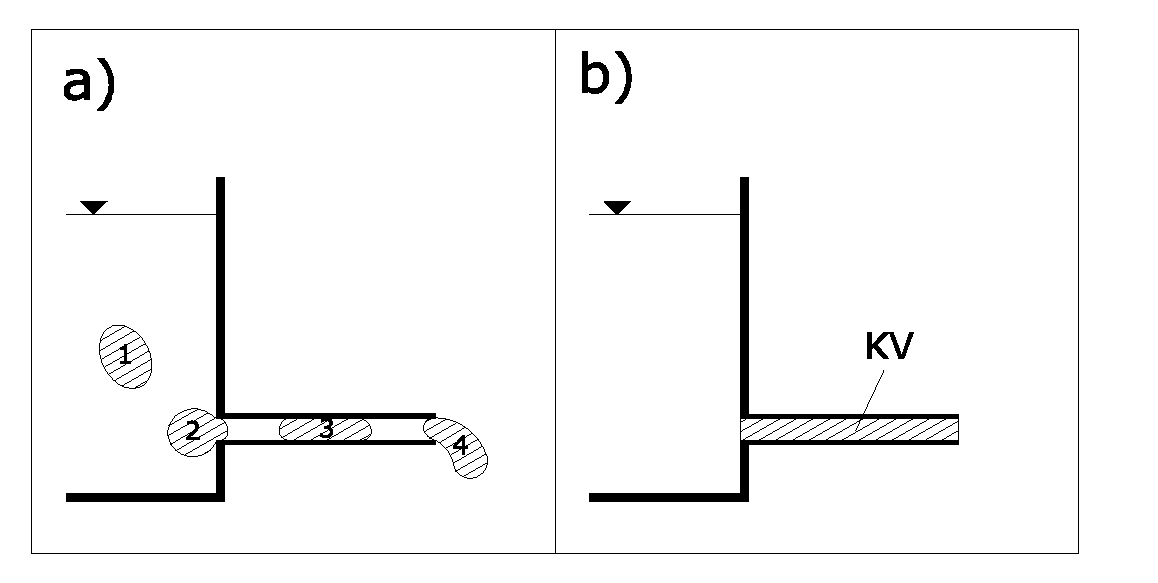
\includegraphics[width=0.8\paperwidth]{figs/slika-mat-vs-kont}
\par\end{centering}
\caption{a) Materijalni volumen tekućine u 4 vremenska trenutka: pratimo točno
određeni volumen tekućine pri istjecanju iz rezervoara. b) Interesira
nas što se događa u cijevi --- volumen cijevi je kontrolni volumen.}
\end{figure}
\end{frame}

\begin{frame}{Protok}

\begin{figure}
\includegraphics[scale=0.3]{figs/protok}\caption{Mjerenje protoka}
\end{figure}
\end{frame}

\begin{frame}{Protok}

\begin{alertblock}{Srednji volumni protok}
Volumen fluida koji u jediničnom vremenu prođe kroz cijev
\[
Q\equiv\frac{\Delta V}{\Delta t}
\]
\end{alertblock}

\begin{block}{Trenutni volumni protok}
\[
Q=\lim_{\Delta t\rightarrow0}\frac{\Delta V}{\Delta t}=\frac{dV}{dt}
\]
\end{block}

\begin{block}{Trenutni maseni protok}
\[
Q_{m}=\dot{m}=\lim_{\Delta t\rightarrow0}\frac{\Delta m}{\Delta t}=\frac{dm}{dt}
\]
\end{block}
\end{frame}

\begin{frame}{Protok kroz cijev površine presjeka $S$}

\begin{figure}
\includegraphics[scale=0.25]{figs/protok-kroz-cijev}
\end{figure}
\[
Q=\lim_{\Delta t\rightarrow0}\frac{\Delta V}{\Delta t}=\lim_{\Delta t\rightarrow0}\frac{S\Delta r}{\Delta t}=S\lim_{\Delta t\rightarrow0}\frac{\Delta r}{\Delta t}=S\frac{dr}{dt}=Sv
\]
\end{frame}

\begin{frame}{Protok kroz proizvoljnu plohu $\varOmega$}

\begin{itemize}
\item u najopćenitijem slučaju kad brzina nije okomita na plohu i nije ista
u svim točkama plohe ukupni volumni protok kroz plohu $\varOmega$
možemo izračunati integracijom
\[
Q_{_{\varOmega}}\equiv\int\limits _{\;\varOmega}\!\!\!\!\!\int\vec{v}\cdot d\vec{S}\quad\quad[\frac{m^{3}}{s}]
\]
\item korisno je uvesti pojam \textbf{srednje brzine} kroz plohu $\varOmega$
\[
\bar{v}\equiv\frac{Q_{_{\varOmega}}}{S}=\frac{1}{S}\int\limits _{\;\varOmega}\!\!\!\!\!\int\vec{v}\cdot d\vec{S}\quad\quad[\frac{1}{m^{2}}\cdot\frac{m^{3}}{s}=\frac{m}{s}]
\]
\item u slučaju kad je $S$ površina presjeka cijevi $\bar{v}$ je srednja
brzina tečenja kroz cijev
\end{itemize}
\end{frame}

\begin{frame}{Jednadžba kontinuiteta za nestlačivi fluid}

\begin{figure}
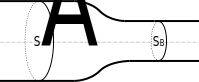
\includegraphics[scale=1.35]{figs/jdba-kont-cijev}
\end{figure}
\[
Q_{A}=Q_{B}\;\Rightarrow\;\bar{v}_{A}S_{A}=\bar{v}_{B}S_{B}
\]
\end{frame}

\begin{frame}{Na manjem presjeku brzina je veća!}

\begin{figure}
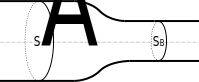
\includegraphics[scale=1.35]{figs/jdba-kont-cijev}
\end{figure}
 \[
\bar{v}_{A}S_{A}=\bar{v}_{B}S_{B}\;\Rightarrow\;\bar{v}_{B}=\frac{S_{A}}{S_{B}}\bar{v}_{A}\;\Rightarrow\;\bar{v}_{B}>\bar{v}_{A}
\]
\end{frame}


\section{Vektorska polja brzine i ubrzanja}

\begin{frame}{Vektorska polja brzine i ubrzanja}

U Eulerovom pristupu fluid je opisan poljima --- temperatura i tlak
su skalarna polja u svakoj točki prostora koji je ispunjen fluidom,
a vektori brzine i ubrzanja čine vektorska polja brzine i ubrzanja
koja su međusobno povezana očekivanom relacijom
\[
\vec{a}(x,y,z,t)=\frac{d\vec{v}(x,y,z,t)}{dt}
\]
U skladu s teorijom funkcija više varijabli totalni diferencijal polja
brzine je
\[
d\vec{v}(x,y,z,t)=\frac{\partial\vec{v}}{\partial x}dx+\frac{\partial\vec{v}}{\partial y}dy+\frac{\partial\vec{v}}{\partial z}dz+\frac{\partial\vec{v}}{\partial t}dt
\]
pa je polje ubrzanja
\[
\vec{a}(x,y,z,t)=v_{x}\frac{\partial\vec{v}}{\partial x}+v_{y}\frac{\partial\vec{v}}{\partial y}+v_{z}\frac{\partial\vec{v}}{\partial z}+\frac{\partial\vec{v}}{\partial t}=(\vec{v}\cdot\vec{\nabla})\vec{v}+\frac{\partial\vec{v}}{\partial t}
\]
\end{frame}

\begin{frame}{Lokalno ubrzanje}

\begin{block}{Lokalno ubrzanje}
Član $\frac{\partial\vec{v}}{\partial t}$ različit je od nule ako
se polje brzine mijenja u vremenu i naziva se \textbf{lokalno ubrzanje}.
\end{block}
\begin{alertblock}{Stacionarno tečenje}
Ako nema promjene brzine u vremenu, tj. brzina u svakoj pojedinoj
točki prostora (kontrolnog volumena) ostaje stalna i ne mijenja se
u vremenu (pri čemu je brzina općenito različita u različitim točkama
prostora!) tečenje je \textbf{stacionarno }i vrijedi
\[
\frac{\partial\vec{v}}{\partial t}=0
\]
\end{alertblock}
\end{frame}

\begin{frame}{Prijenosno (konvektivno) ubrzanje}

Preostali članovi polja ubrzanja koji ne ovise eksplicitno o vremenu
\[
v_{x}\frac{\partial\vec{v}}{\partial x}+v_{y}\frac{\partial\vec{v}}{\partial y}+v_{z}\frac{\partial\vec{v}}{\partial z}=(\vec{v}\cdot\vec{\nabla})\vec{v}
\]
nazivaju se \textbf{prijenosno ili konvektivno ubrzanje}.
\begin{block}{}
Dakle, čak i u slučaju stacionarnog tečenja, kad se polje brzine
ne mijenja u vremenu, pojedine čestice fluida se na svojoj putanji
mogu ubrzavati i usporavati, ovisno o tome u kojoj točki polja se
nalaze.
\end{block}
\end{frame}

\section{Izvod Bernoullijeve jednadžbe}

\begin{frame}{Osnovna jednadžba hidrostatike}

Iz uvjeta ravnoteže površinskih i volumenskih sila 
\[
\sum\vec{F}_{S}+\sum\vec{F}_{V}=\vec{0}
\]
koje djeluju na mali volumen fluida $\Delta V=\Delta x\,\Delta y\,\Delta z$
\[
-\vec{\nabla}p\:\Delta V+\rho\,\vec{g}_{ef}\,\Delta V=\vec{0}
\]
izvedena je osnovna jednadžba hidrostatike
\[
\vec{\nabla}p=\rho\,\vec{g}_{ef}
\]
\end{frame}

\begin{frame}{Eulerova jednadžba}

Ako površinske i volumenske sile nisu u ravnoteži onda mora vrijediti
2. Newtonov zakon
\[
\sum\vec{F}_{S}+\sum\vec{F}_{V}=m\vec{a}
\]
to jest
\[
-\vec{\nabla}p\:\Delta V+\rho\,\vec{g}_{ef}\,\Delta V=\rho\:\Delta V\:\vec{a}
\]
pri čemu je $\vec{a}(x,y,z,t)$ polje ubrzanja koje se sastoji od
prijenosnog i lokalnog ubrzanja pa slijedi
\[
-\vec{\nabla}p+\rho\,\vec{g}_{ef}=\rho[(\vec{v}\cdot\vec{\nabla})\vec{v}+\frac{\partial\vec{v}}{\partial t}]
\]
i to je \textbf{Eulerova dinamička jednadžba za strujanje idealne
(neviskozne) tekućine}
\end{frame}

\begin{frame}{Rješavanje Eulerove jednadžbe}

Rješavanje Eulerove jednadžbe je veoma složeno pa ćemo se ograničiti
na \textbf{stacionarno strujanje }u polju sile teže ($\vec{g}_{ef}=-g\,\vec{k}$)
\[
-\vec{\nabla}p+\rho\,\vec{g}=\rho\:(\vec{v}\cdot\vec{\nabla})\vec{v}
\]
Matematičkim manipulacijama moguće je taj izraz preformulirati u
\[
\vec{\nabla}p+\rho g\vec{k}+\frac{1}{2}\rho\vec{\nabla}(v^{2})=\rho[\vec{v}\times(\vec{\nabla}\times\vec{v})]
\]
Ako se taj izraz pomnoži s malim pomakom duž putanje (strujnice) $d\vec{r}$
desna strana izraza će zbog svojstva skalarnog produkta (produkt okomitih
vektora je nula!) biti nula i ostaje 
\[
\vec{\nabla}p\cdot d\vec{r}+\rho g\vec{k}\cdot d\vec{r}+\frac{1}{2}\rho\vec{\nabla}(v^{2})\cdot d\vec{r}=0
\]
\end{frame}

\begin{frame}{Projekcija na strujnicu}

Uvažavajući 
\[
d\vec{r}=dx\:\vec{i}+dy\:\vec{j}+dz\:\vec{k}
\]
i definiciju gradijenta dobije se 
\[
\vec{\nabla}p\cdot d\vec{r}=\frac{\partial p}{\partial x}dx+\frac{\partial p}{\partial y}dy+\frac{\partial p}{\partial z}dz=dp
\]
tj. totalni diferencijal od $p$. Isto tako je $\vec{\nabla}(v^{2})\cdot d\vec{r}$
totalni diferencijal od $v^{2}$, a $\vec{k}\cdot d\vec{r}=dz$ zbog
ortogonalnost jediničnih vektora $\vec{i}$, $\vec{j}$ i $\vec{k}$.
Rezultat 
\[
dp+\rho gdz+\frac{1}{2}\rho d(v^{2})=0
\]
je projekcija Eulerove jednadžbe na strujnicu.
\end{frame}

\begin{frame}{Bernoullijeva jednadžba}

Dobiveni izraz koji se sastoji samo od totalnih diferencijala može
se lako integrirati duž strujnice, od neke točke $A$ do točke $B$
\[
\int\limits _{A}^{B}dp+\int\limits _{A}^{B}\rho g\,dz+\frac{1}{2}\int\limits _{A}^{B}\rho\,d(v^{2})=0
\]
i ako uzmemo da su stvarne tekućine praktički nestlačive ($\rho=konst.)$,
integracijom (i preslagivanjem) dobije se 
\[
p_{{\scriptscriptstyle A}}+\rho gz_{{\scriptscriptstyle A}}+\frac{1}{2}\rho v_{{\scriptscriptstyle A}}^{2}=p_{{\scriptscriptstyle B}}+\rho gz_{{\scriptscriptstyle B}}+\frac{1}{2}\rho v_{{\scriptscriptstyle B}}^{2}
\]
Kako je izbor točaka $A$ i $B$ na strujnici bio proizvoljan, mora
vrijediti 
\[
p+\rho gz+\frac{1}{2}\rho v^{2}=konst.
\]
za sve točke duž strujnice i to je \textbf{\textcolor{red}{Bernoullijeva
jednadžba}}.
\end{frame}

\begin{frame}{Ograničenja u primjeni Bernoullijeve jednadžbe}

\begin{alertblock}{Ograničenja u primjeni Bernoullijeve jednadžbe}
Zbog pojednostavljenja i aproksimacija koje su načinjene tijekom
izvoda primjena Bernoullijeve jednadžbe je ograničena na slučajeve
kad su istovremeno ispunjeni svi ovi ograničavajući uvjeti 

\begin{itemize}
\item neviskozno tečenje, to jest tečenje sa zanemarivim unutarnjim trenjem 
\item stacionarno tečenje ($\frac{\partial\vec{v}}{\partial t}=0$) 
\item nestlačivi fluid ($\rho=konst.$) 
\item tečenje duž strujnice. 
\end{itemize}

\end{alertblock}
Napomena: U specijalnom slučaju takozvanog bezvrtložnog polja brzina
(kad je ispunjen uvjet $\vec{\nabla}\times\vec{v}=0$) valjanost Bernoullijeve
jednadžbe nije ograničena samo duž strujnice.
\end{frame}

\section{Bernoullijeva jednadžba}

\begin{frame}{Tlačni oblik Bernoullijeve jednadžbe}

U fizici je uobičajen zapis Bernoullijeve jednadžbe
\[
p+\rho gz+\frac{1}{2}\rho v^{2}=konst.
\]
Taj oblik naziva se \textbf{\textcolor{red}{tlačni}} jer svi članovi
imaju dimenziju tlaka i mjere se u paskalima:
\begin{eqnarray*}
[p] & = & Pa\\
{}[\rho gz] & = & [\rho][g][z]=\frac{kg}{m^{3}}\frac{m}{s^{2}}m=\frac{N}{m^{2}}=Pa\\
{}[\frac{1}{2}\rho v^{2}] & = & [\rho][v]^{2}=\frac{kg}{m^{3}}\frac{m^{2}}{s^{2}}=\frac{N}{m^{2}}=Pa.
\end{eqnarray*}
\end{frame}

\begin{frame}{Hidraulički, hidrostatički i dinamički tlak}

Suma tri člana duž strujnice je konstantna
\[
p+\rho gz+\frac{1}{2}\rho v^{2}=konst.
\]
\begin{block}{Pojedini članovi imaju svoje nazive:}
\begin{description}
\item [{$\rho gz$}] je već poznati \textcolor{red}{\emph{hidrostatički
tlak}}
\item [{$\frac{1}{2}\rho v^{2}$}] naziva se \textcolor{red}{\emph{dinamički
tlak}} jer ovisi o brzini (zapravo bi precizniji naziv bio \emph{kinematički
tlak})
\item [{$p$}] je \textcolor{red}{\emph{hidraulički tlak}}
\end{description}
\end{block}
\end{frame}

\begin{frame}{Fizikalna interpretacija}

Dinamički tlak
\[
\frac{1}{2}\rho v^{2}
\]
nesumnjivo podsjeća na izraz za kinetičku energiju tijela mase $m$
koje se giba brzinom $v$
\[
E_{k}=\frac{1}{2}mv^{2}
\]
S obzirom da je $\rho=\frac{m}{V}$ slijedi da je
\[
\frac{1}{2}\rho v^{2}=\frac{\frac{1}{2}mv^{2}}{V}=\frac{E_{k}}{V}
\]
tj. \textcolor{red}{\emph{kinetička energija po jediničnom volumenu
tekućine}}.
\end{frame}

\begin{frame}{Fizikalna interpretacija}

Isto vrijedi i za hidrostatički tlak
\[
\rho gz
\]
koji podsjeća na izraz za potencijalnu energiju u polju sile teže
\[
E_{p,G}=mgz
\]
S obzirom da je $\rho=\frac{m}{V}$ slijedi da je
\[
\rho gz=\frac{mgz}{V}=\frac{E_{p,G}}{V}
\]
tj. \textcolor{red}{\emph{potencijalna energija sile teže po jediničnom
volumenu tekućine}}.

\end{frame}

\begin{frame}{Specifična energija po jedinici volumena tekućine}

\begin{alertblock}{Fizikalna interpretacija}
 Članovi u tlačnom obliku Bernoullijeve jednadžbe predstavljaju \textbf{specifičnu
energiju po jedinici volumena tekućine}.
\end{alertblock}

Ta interpretacija nije u kontradikciji sa činjenicom da se članovi
mjere u paskalima, jer je
\[
Pa=\frac{N}{m^{2}}=\frac{N}{m^{2}}\cdot\frac{m}{m}=\frac{Nm}{m^{3}}=\frac{J}{m^{3}}.
\]
\emph{Paskal} možemo interpretirati kao \emph{džul po kubnom metru},
tj. kao mjeru za \textcolor{black}{\emph{energiju po jediničnom volumenu}}.
\end{frame}

\begin{frame}{Fizikalna interpretacija hidrauličkog tlaka}

\begin{itemize}
\item volumen tekućina se pod tlakovima koji nisu mnogo veći od atmosferskog
tek neznatno smanjuje (\emph{tekućine su praktički nestlačive!})
\item u proračunima se uzima da su volumen, a time i gustoća tekućina, konstantni
\item ipak, tekućine jesu stlačive i u stlačenoj tekućini pohranjena je
elastična potencijalna energija --- kao što je pohranjena i u stlačenoj
opruzi
\end{itemize}

\begin{block}{}
Hidraulički tlak $p$ odgovara \textbf{\textcolor{red}{specifičnoj
elastičnoj potencijalnoj energiji po jedinici volumena tekućine}}
koja je stlačena pod tim tlakom.
\end{block}
\end{frame}

\begin{frame}{Specifična energija po jedinici mase}

\begin{itemize}
\item kad se koristi naziv \emph{specifična energija} bez da se spomene
da se odnosi na jedinični volumen obično se podrazumijeva da se radi
o \emph{energiji po jediničnoj masi}
\item jednostavno je Bernoullijevu jednadžbu iz tlačnog oblika preoblikovati
tako da pojedini članovi predstavljaju \emph{specifičnu energiju po
jedinici mase}: jednadžbu treba podijeliti s gustoćom tekućine $\rho$
\[
p+\rho gz+\frac{1}{2}v^{2}=konst.\quad/:\rho
\]
\[
\frac{p}{\rho}+gz+\frac{1}{2}v^{2}=\frac{konst.}{\rho}=\mathcal{E}
\]
\end{itemize}
\end{frame}

\begin{frame}{Specifična energija po jedinici mase}

\begin{itemize}
\item kad se podijeli s gustoćom $\rho$ energija po jediničnom volumenu
postaje energija po jedinici mase
\[
\frac{E}{V}\;:\;\rho=\frac{E}{\rho V}=\frac{E}{m}
\]
\item izraženo mjernim jedinicama
\[
\frac{J}{m^{3}}\;:\;\frac{kg}{m^{3}}=\frac{J}{m^{3}}\:\frac{m^{3}}{kg}=\frac{J}{kg}
\]
\item ovaj oblik Bernoullijeve jednadžbe se u praksi relativno rijetko koristi
i nema neko posebno ime
\end{itemize}
\end{frame}

\begin{frame}{Visinski oblik Bernoullijeve jednadžbe}

\begin{itemize}
\item osim sa gustoćom $\rho$ tlačni oblik Bernoullijeve jednadžbe može
se podijeliti i s ubrzanjem slobodnog pada $g$ 
\[
p+\rho gz+\frac{1}{2}\rho v^{2}=konst.\quad/:(\rho g)
\]
\item dobije se oblik u kojem pojedini članovi imaju dimenziju duljine,
tj. mjere se u metrima
\[
\frac{p}{\rho g}+z+\frac{v^{2}}{2g}=H
\]
\item postavlja se pitanje fizikalne interpretacije?
\end{itemize}
\end{frame}

\begin{frame}{Visinski oblik Bernoullijeve jednadžbe}

\begin{itemize}
\item ako specifičnu energiju po jedinici volumena podijelimo i sa $\rho$
i sa $g$ slijedi
\[
\frac{E}{V}\;:\;\rho\;:\;g=\frac{E}{\rho V}\;:\;g=\frac{E}{m}\;:\;g=\frac{E}{mg}=\frac{E}{G}
\]
\item nameće se očigledna interpretacija da se u ovom slučaju radi o \textcolor{red}{\emph{specifičnoj
energiji po jedinici težine tekućine}}
\item lako je pokazati da je metar ekvivalentan džulu po njutnu
\[
m=m\cdot\frac{N}{N}=\frac{Nm}{N}=\frac{J}{N}
\]
\end{itemize}
\end{frame}

\begin{frame}{Visinski oblik Bernoullijeve jednadžbe}

\textbf{\textcolor{red}{Visinski oblik}} Bernoullijeve jednadžbe je
\[
\frac{p}{\rho g}+z+\frac{v^{2}}{2g}=H
\]
\begin{block}{Pojedini članovi imaju svoje nazive:}
\begin{description}
\item [{$\frac{p}{\rho g}$}] je\textcolor{red}{\emph{ tlačna visina }}\textcolor{black}{\emph{(engl.
pressure head)}}
\item [{$z$}] je \textcolor{red}{\emph{geodetska visina }}\textcolor{black}{\emph{(engl.
elevation head)}}
\item [{$\frac{v^{2}}{2g}$}] je \textcolor{red}{\emph{brzinska visina
}}\textcolor{black}{\emph{(engl. velocity head)}}
\item [{$H$}] je \textcolor{red}{\emph{ukupna energijska visina}} \emph{(engl.
total head)}
\end{description}
\end{block}
\end{frame}

\begin{frame}{Piezometarska visina}

\begin{itemize}
\item tlačna visina u metrima može se interpretirati kao visina stupca tekućine
gustoće $\rho$ u polju sile teže jakosti $g$ uslijed kojeg nastaje
tlak $p$
\item geodetska visina $z$ mjeri se u odnosu na referentnu ravninu
\item odabir referentne ravnine je zapravo proizvoljan
\item suma tlačne i geodetske visine naziva se \textcolor{red}{\emph{piezometarska
visina }}\emph{(engl. piezometric head)}
\[
\Pi=\frac{p}{\rho g}+z
\]
\item taj naziv motiviran je činjenicom da je to upravo ona visina (u odnosu
na referentnu ravninu) koja se očitava na piezometru
\end{itemize}
\end{frame}

\begin{frame}{Piezometar}

\begin{figure}
%\includegraphics[width=1\textwidth]{primjenaBJ/piezometar}
\end{figure}
\end{frame}

\section{Primjena Bernoullijeve jednadžbe}

\begin{frame}{Pitotova cijev}

\begin{figure}
%\includegraphics[width=1\textwidth]{primjenaBJ/MF-06-BJ-2015_7}
\end{figure}
\end{frame}

\begin{frame}{Venturijeva cijev}

\begin{figure}
%\includegraphics[width=1\textwidth]{primjenaBJ/MF-06-BJ-2015_8}
\end{figure}
\end{frame}

\begin{frame}{Venturijeva cijev}

\begin{figure}
%\includegraphics[width=1\textwidth]{primjenaBJ/MF-06-BJ-2015_9}
\end{figure}
\end{frame}

\begin{frame}{Venturijeva cijev}

\begin{figure}
%\includegraphics[width=1\textwidth]{primjenaBJ/MF-06-BJ-2015_10}
\end{figure}
\end{frame}

\begin{frame}{Torricellijev zakon}

\begin{figure}
%\includegraphics[width=1\textwidth]{primjenaBJ/MF-06-BJ-2015_11}
\end{figure}
\end{frame}

\begin{frame}{Torricellijev zakon}

\begin{figure}
%\includegraphics[width=1\textwidth]{primjenaBJ/MF-06-BJ-2015_12}
\end{figure}
\end{frame}

\end{document}
